\documentclass[autodetect-engine,dvi=dvipdfmx,ja=standard,
               a4j,11pt]{bxjsarticle}

\RequirePackage{geometry}
\geometry{reset,paperwidth=210truemm,paperheight=297truemm}
\geometry{hmargin=.75truein,top=20truemm,bottom=25truemm,footskip=10truemm,headheight=0mm}
%\geometry{showframe} % 本文の"枠"を確認したければ,コメントアウト
\usepackage{graphicx}
\usepackage{subcaption}
\usepackage{fancyvrb}
\usepackage{spverbatim}
\usepackage{amsmath}
\renewcommand{\theFancyVerbLine}{\texttt{\footnotesize{\arabic{FancyVerbLine}:}}}

\title{画像処理実験 第5回}
\author{学生番号: 09B23523\\
        大野颯也 (OHNO, Soya)}
\date{\number\year 年\number\month 月\number\day 日}

%%======== 本文 ====================================================%%
\begin{document}
\maketitle
% 目次つきの表紙ページにする場合はコメントを外す
%{\footnotesize \tableofcontents \newpage}


%--------------------------------------------------------------------%
%\begin{Verbatim}[numbers=left, xleftmargin=10mm, numbersep=6pt,
%                    fontsize=\small, baselinestretch=0.8]
%def main():
%  s=[ord('A'), ord('B'), ord('C')]
%  print(s)
%  print(bytes(s).decode())
%\end{Verbatim}

%--------------------------------------------------------------------%
%\section{数式: 行列,ベクトル}

%\newcommand\bA{\mbox{\boldmath$A$}}
%\newcommand\bb{\mbox{\boldmath$b$}}
%太字$\bA$を使えるように定義した.
%$\bA^{-1}\bb$等,使う文字を newcommand で定義して使う.

% \boldsymbol{A} は使えない


%--------------------------------------------------------------------%




%--------------------------------------------------------------------%
\section{第5回} \label{sec:abstract}
\subsection{課題5.2}
\subsubsection{極大点リストから,「特徴点らしさ」の大きいものを MAX 個選び出す}
大きいものから選び出す必要があるため, ary をソートする.以下がソートに使用した関数である.

\begin{Verbatim}[numbers=left, xleftmargin=10mm, numbersep=6pt,
                    fontsize=\small, baselinestretch=0.8]
def quicksort_des(ary,low,high):
  if low>=high:
    return
  pivot=ary[(low+high)//2,2]
  i,j=low,high
  while i<=j:
    while ary[i,2]>pivot:
      i+=1
    while ary[j,2]<pivot:
      j-=1
    if i<=j:
      ary[i,:],ary[j,:]=ary[j,:].copy(),ary[i,:].copy()
      i+=1
      j-=1
  quicksort_des(ary,low,j)
  quicksort_des(ary,i,high)
\end{Verbatim}

Python では値を渡すことができず,代入渡しとなってしまうため,swap関数部分である

\begin{Verbatim}[numbers=left, xleftmargin=10mm, numbersep=6pt,
                    fontsize=\small, baselinestretch=0.8]
      ary[i,:],ary[j,:]=ary[j,:].copy(),ary[i,:].copy()
\end{Verbatim}

では .copy() を使用して,値のみを変換するようにしている.

MAX は detectFeaturePoints関数 に引数として渡されているため,

\begin{Verbatim}[numbers=left, xleftmargin=10mm, numbersep=6pt,
                    fontsize=\small, baselinestretch=0.8]
  quicksort_des(ary,0,len(x)-1)
  ary=ary[:MAX]
\end{Verbatim}

と記述することで大きいものから MAX 個選ぶことができる.


\subsection{課題5.3}
\subsubsection{LocalMax の説明}
LocalMax 関数は次のようになっている.

\begin{Verbatim}[numbers=left, xleftmargin=10mm, numbersep=6pt,
                    fontsize=\small, baselinestretch=0.8]
def LocalMax(src,W=7):
# (5) 近傍での最大値検出
  out=np.zeros_like(src)
  for v in range(-W,W+1):
   for u in range(-W,W+1):
    out[W:-W,W:-W]=np.maximum(out[W:-W,W:-W],
                              src[v+W:src.shape[0]+v-W,
                                  u+W:src.shape[1]+u-W])
  return out
\end{Verbatim}

この関数は,点[y,x] について周囲[W:-W,W:-W]における最大値に値を置き換えるという作業を (u,v) をずらしながら行う.図\ref{fig:5.2_TKfilter.png},\ref{fig:5.2_LocalMax.png}はそれぞれ TKfilter によって絞られた特徴点の候補,LocalMax によってある特徴点候補における周辺$15 \times 15$における最大値である.

\begin{figure}[h]
 \centering
 \begin{subfigure}[b]{0.45\textwidth}
   \centering
   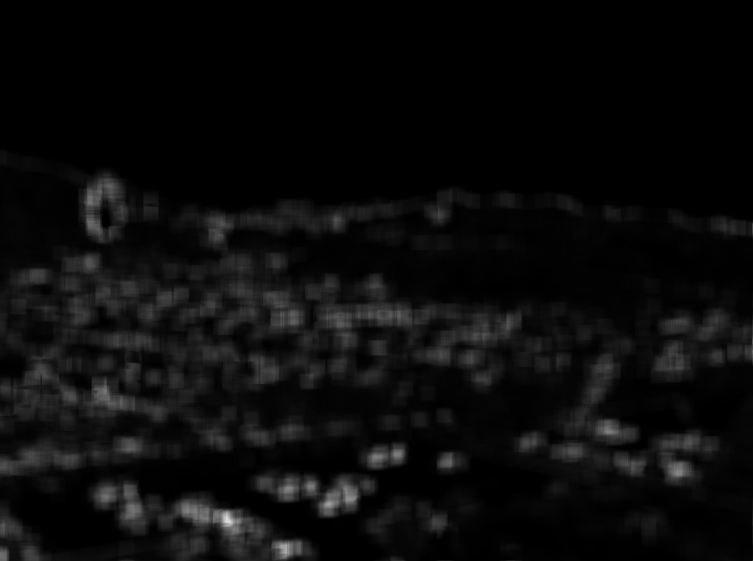
\includegraphics[scale=0.2]{5.2_TKfilter.png}
   \caption{TKfilter後の画像}
   \label{fig:5.2_TKfilter.png}
 \end{subfigure}
 \hspace{5mm}
 \begin{subfigure}[b]{0.45\textwidth}
   \centering
   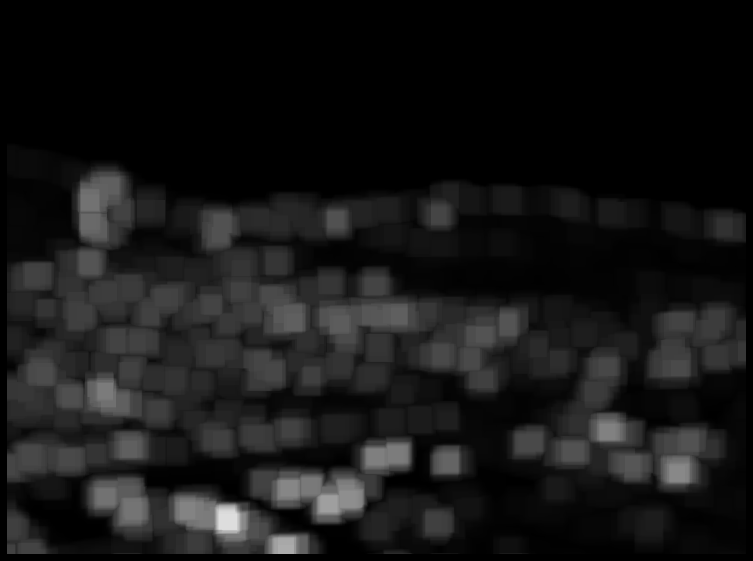
\includegraphics[scale=0.2]{5.2_LocalMax.png}
   \caption{LocalMax後の画像}
   \label{fig:5.2_LocalMax.png}
 \end{subfigure}
 \caption{LocalMax による画像の変化}
 \label{fig:comparison_W}
\end{figure}

blur 関数では周囲[W:-W,W:-W]の平均値を出していたので,処理は加算をするところを最大値を取得するように置き換えただけで実装できる.


\subsubsection{縦横2段階に分解して効率化}
以下は縦と横の二段階にして効率化したものである.

\begin{Verbatim}[numbers=left, xleftmargin=10mm, numbersep=6pt,
                    fontsize=\small, baselinestretch=0.8]
def LocalMax(src,W=7):
 out=np.zeros_like(src)
 T=np.zeros_like(src)
 for v in range(-W,W+1):
  T[W:-W,W:-W]=np.maximum(T[W:-W,W:-W],
                          src[v+W:v+src.shape[0]-W,
                              W:src.shape[1]-W])
 for u in range(-W,W+1):
  out[W:-W,W:-W]=np.maximum(out[W:-W,W:-W],
                            T[W:-W,u+W:u+src.shape[1]-W])
 return out
\end{Verbatim}

次が,(1)デフォルト (2)効率化後 の実行速度である.

\begin{Verbatim}[numbers=left, xleftmargin=10mm, numbersep=6pt,
                    fontsize=\small, baselinestretch=0.8]
(1) Max:0.207 sec
(2) Max:0.036 sec
\end{Verbatim}

6倍程度高速に動いていることがわかる.これは blur においてもそうだったが,二重ループによって $15^2$ 回の処理が必要だったものを,ループを2段階に分けることによって $15 \times 2$ 回の処理で済んでいるからである.


\subsubsection{FASTとNAIVEの速度・結果を比較}
極大判定における,FAST な実装と NAIVE な実装について比較する.

\begin{Verbatim}[numbers=left, xleftmargin=10mm, numbersep=6pt,
                    fontsize=\small, baselinestretch=0.8]
(1) ary:0.002 sec
(2) ary:0.160 sec
\end{Verbatim}
(1) が FAST な実装で,(2) が NAIVE な実装である.ここまでの速度の差が出てきてしまっているのは, FAST においては行列式の計算を行っているのに対し, NAIVE においては二重ループの計算 ($1024 \times 768$) を行っているからである.

FAST で行っていることは,0の要素を省いて計算することである.厳密には,数値が0でない値(0以上)に対してその座標と値を行列として集めている.これによって高速な処理を可能にしている.以下において,np.where などの使い方を載せる.

\begin{Verbatim}[numbers=left, xleftmargin=10mm, numbersep=6pt,
                    fontsize=\small, baselinestretch=0.8]
  X=np.array([0,2,0,0,3])
  idx = np.where(X)[0]
  vals = X[idx]
  Mat = np.array([idx, vals])
  print(Mat)
  Mat=Mat.T
  print(Mat)

---------- 実行結果 ----------

[[1 4]
 [2 3]]
[[1 2]
 [4 3]]
\end{Verbatim}



\subsubsection{全体のコード}
\begin{Verbatim}[numbers=left, xleftmargin=10mm, numbersep=6pt,
                    fontsize=\small, baselinestretch=0.8]
# [5.1 features]

def LocalMax(src,W=7):
 out=np.zeros_like(src)
 T=np.zeros_like(src)
 for v in range(-W,W+1):
  T[W:-W,W:-W]=np.maximum(T[W:-W,W:-W],
                          src[v+W:v+src.shape[0]-W,
                              W:src.shape[1]-W])
 for u in range(-W,W+1):
  out[W:-W,W:-W]=np.maximum(out[W:-W,W:-W],
                            T[W:-W,u+W:u+src.shape[1]-W])
 return out


def detectFeaturePoints(src,MAX=100):
  W=7

  tkf=TKfilter(src)
  eb.                stopWatch('TKfilter')
  out=LocalMax(tkf)
  out[    :W+1]=0    # 周辺 8 pixel は除去
  out[-W-1:   ]=0    # ※1
  out[:,    :W+1]=0
  out[:,-W-1:   ]=0
  eb.                stopWatch('Max')

# (6) 極大判定
## FAST:
  mask=(out==tkf)&(out>0) # (最大値 == 中心) かつ (最大値 > 0)
  y,x=np.where(mask)      # mask[y,x]!=0 であるような x,y のリスト
  ary=np.vstack((x,y,out[y,x])).T # [x,y,out[y,x]] を行とする行列

## NAIVE:
#  hgt,wdt=tkf.shape
#  ary=[]
#  for y in range(W+1,hgt-W-1):
#   for x in range(W+1,wdt-W-1):
#    if out[y,x]==tkf[y,x] and out[y,x]>0:
#     ary+=[[x,y,out[y,x]]]
#  ary=np.array(ary)

  eb.                stopWatch('ary')

  # (7) ary を第3列の降順に MAX 個残す
  quicksort_des(ary,0,len(ary)-1)
  ary=ary[:MAX]
  eb.                stopWatch('sort')

  # (8) 画像で結果表示
  hgt,wdt=tkf.shape
  img=np.zeros((hgt,wdt,3),'f') # 出力画像
  img[:,:,0]=tkf*9 # 濃淡画像からカラー画像に変換
  img[:,:,1]=tkf*9 # Numpy tips: Broadcast を参照
  img[:,:,2]=tkf*9

  for x,y,v in ary:
   x=int(x)
   y=int(y)
   img[y-W:y+W+1,x-W:x+W+1]=(img[y-W:y+W+1,x-W:x+W+1]+[1,0,0])/2

  eb.imshow(img)

  return ary


def main():
  src=eb.getImg('0.jpg') # 入力画像
  eb.                      stopWatch('start')
  ary=detectFeaturePoints(src)
  #print(ary)             # ary を表示
  eb.showTime()



def quicksort_des(ary,low,high):
  if low>=high:
    return
  pivot=ary[(low+high)//2,2]
  i,j=low,high
  while i<=j:
    while ary[i,2]>pivot:
      i+=1
    while ary[j,2]<pivot:
      j-=1
    if i<=j:
      ary[i,:],ary[j,:]=ary[j,:].copy(),ary[i,:].copy()
      i+=1
      j-=1
  quicksort_des(ary,low,j)
  quicksort_des(ary,i,high)
\end{Verbatim}

\subsubsection{実行速度}
\begin{Verbatim}[numbers=left, xleftmargin=10mm, numbersep=6pt,
                    fontsize=\small, baselinestretch=0.8]
start:0.005 sec
TKfilter:0.036 sec
Max:0.037 sec
ary:0.002 sec
sort:0.005 sec
\end{Verbatim}


\subsubsection{特徴点が絞られた画像}
\begin{figure}[h]
 \centering
 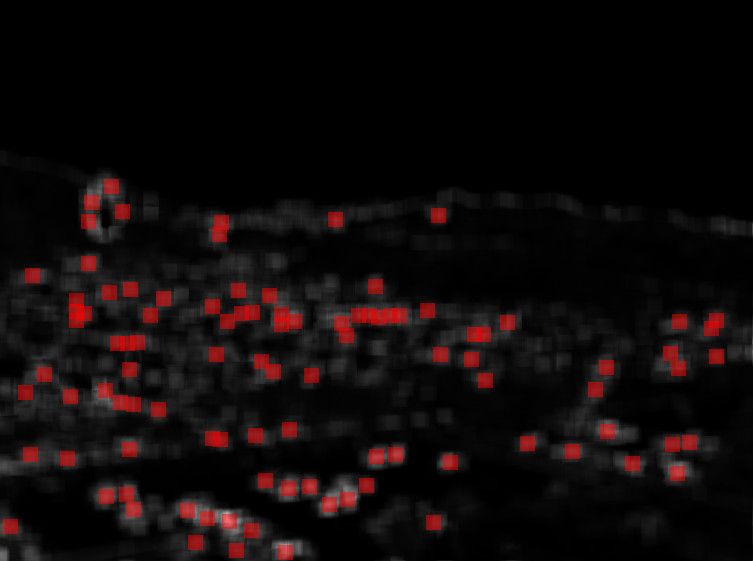
\includegraphics[scale=.5]{5.2_features.jpg}
 \caption{特徴点(周囲15*15)が赤}
 \label{fig:5.2_features.jpg}
\end{figure}


\subsection{自分で撮影した画像}
\begin{figure}[h]
 \centering
 \begin{subfigure}[b]{0.45\textwidth}
   \centering
   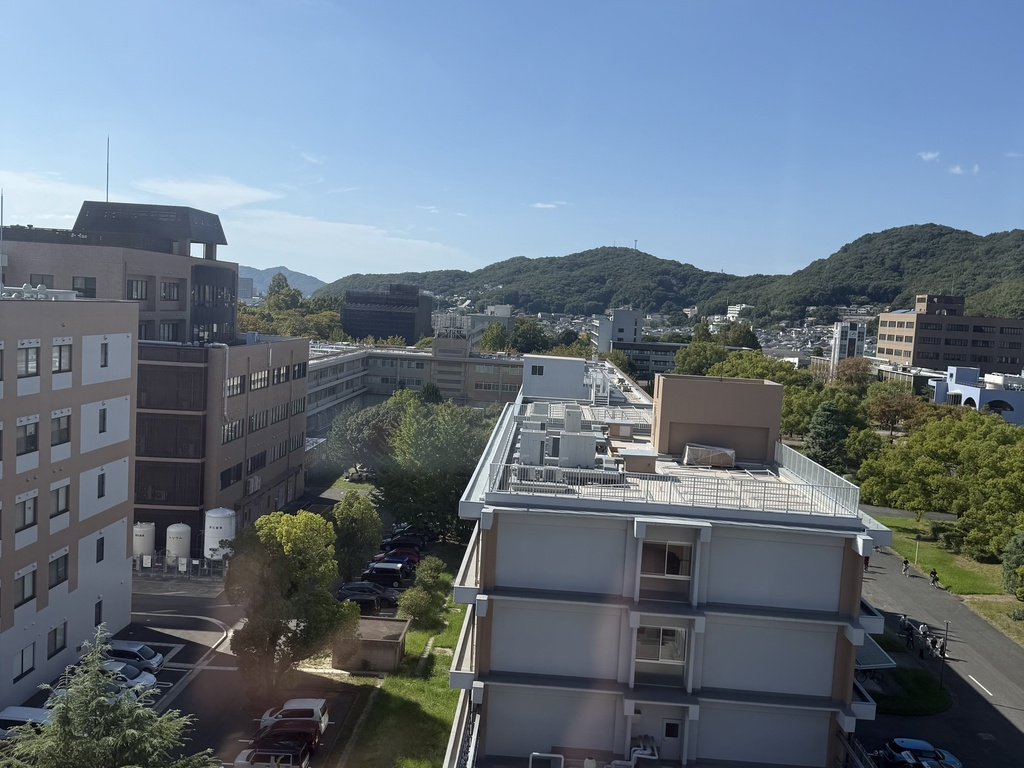
\includegraphics[scale=0.2]{IMG_5566.jpg}
   \caption{撮影した画像}
   \label{fig:5.2_TKfilter.png}
 \end{subfigure}
 \hspace{5mm}
 \begin{subfigure}[b]{0.45\textwidth}
   \centering
   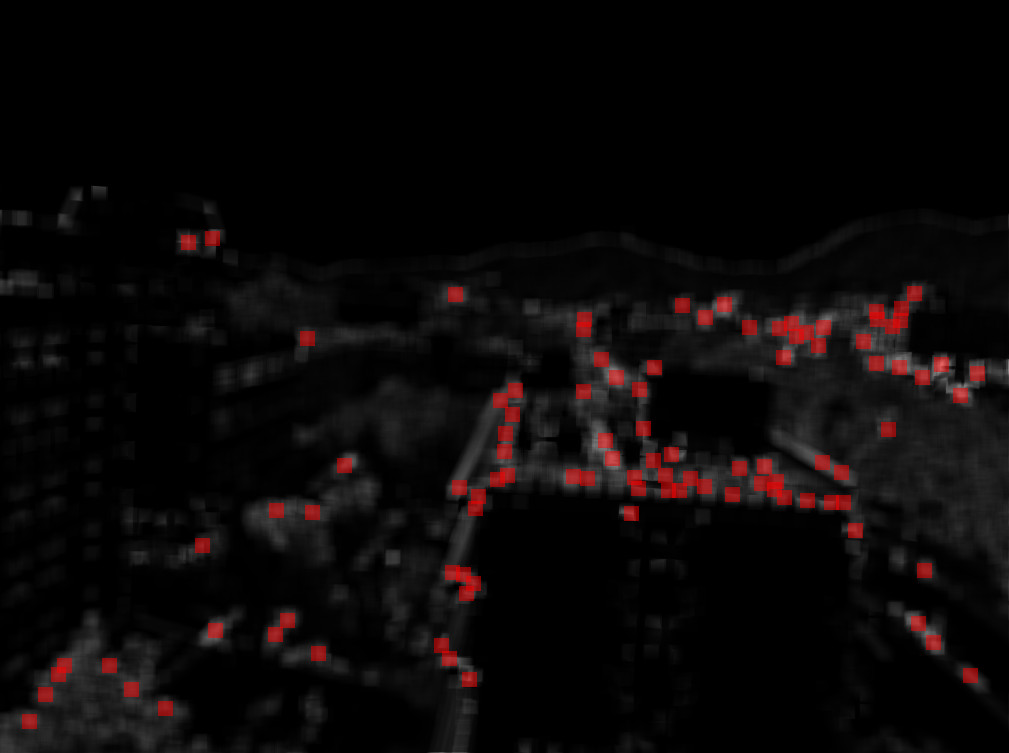
\includegraphics[scale=0.2]{5.3_myfeatures.jpg}
   \caption{特徴点}
   \label{fig:5.2_LocalMax.png}
 \end{subfigure}
 \caption{撮影した画像への実行}
 \label{fig:comparison_W}
\end{figure}

%--------------------------------------------------------------------%
\section{感想}

%--------------------------------------------------------------------%
% 参考文献
%   以下は,書き方の例である.実際に,参考にした書籍等を見て書くこと.
%   本文で引用する際は,\cite{book:algodata}などとすればよい.
%\begin{thebibliography}{99}
%  \bibitem{book:algodata} 平田富雄,アルゴリズムとデータ構造,森北出版,1990.
%  \bibitem{book:label2} 著者名,書名,出版社,発行年.
%  \bibitem{www:label3} WWWページタイトル,\spverb!https://example.of.too.long.url.jp/you.must.use.spverb/and.insert. a.space.somewhere.to.avoid.overfull.html!,アクセス日.
%\end{thebibliography}

%--------------------------------------------------------------------%
\end{document}
